\documentclass[times]{aastex6}

\usepackage{verbatim}
\usepackage{amsmath}

% Spacings between the chapter top and to the text
%\newcommand{\chaptertopspacing}{10}
%\newcommand{\chaptertotextspacing}{-10}
%\newcommand{\chaptertopspacingSTAR}{10}
%\newcommand{\chaptertotextspacingSTAR}{-10}

% Convenience functions
% Paper1
%\DeclareMathOperator*{\argmax}{arg\,max}
%\DeclareMathOperator*{\argmin}{arg\,min}
% Paper2
\newcommand{\Kepler}{Kepler~}
%\newcommand{\KTwo}{K2~}
\newcommand{\MAST}{\textit{MAST\_DR23}}
\newcommand{\Carini}{\textit{CW2015}}
% Paper3
%\DeclareMathOperator{\vect}{vec}
\newcommand{\textbfit}[1]{\textbf{\textit{#1}}}
\newcommand{\mathbfit}[1]{\textbf{\textit{#1}}}
\newcommand{\textbfss}[1]{\textbf{\textsf{#1}}}
\newcommand{\mathbfss}[1]{\textbf{\textsf{#1}}}

\DeclareSymbolFont{UPM}{U}{eur}{m}{n}
\SetSymbolFont{UPM}{bold}{U}{eur}{b}{n}
\DeclareSymbolFont{AMSa}{U}{msa}{m}{n}
\DeclareMathSymbol{\upi}{0}{UPM}{"19}
\DeclareMathSymbol{\umu}{0}{UPM}{"16}
\DeclareMathSymbol{\upartial}{0}{UPM}{"40}
\DeclareMathSymbol{\leqslant}{3}{AMSa}{"36}
\DeclareMathSymbol{\geqslant}{3}{AMSa}{"3E}
\DeclareMathSymbol{\la}{3}{AMSa}{46}
\DeclareMathSymbol{\ga}{3}{AMSa}{38}

\let\oldle=\le     \let\oldleq=\leq
\let\oldge=\ge     \let\oldgeq=\geq
\let\leq=\leqslant \let\le=\leqslant
\let\geq=\geqslant \let\ge=\geqslant

\newcommand\getsto{\mathrel{\mathchoice {\vcenter{\offinterlineskip
\halign{\hfil
$\reset@font\displaystyle##$\hfil\cr\gets\cr\to\cr}}}
{\vcenter{\offinterlineskip\halign{\hfil$\reset@font\textstyle##$\hfil\cr\gets
\cr\to\cr}}}
{\vcenter{\offinterlineskip\halign{\hfil$\reset@font\scriptstyle##$\hfil\cr\gets
\cr\to\cr}}}
{\vcenter{\offinterlineskip\halign{\hfil$\reset@font\scriptscriptstyle##$\hfil\cr
\gets\cr\to\cr}}}}}

\newcommand\cor{\mathrel{\mathchoice {\hbox{$\widehat=$}}{\hbox{$\widehat=$}}
{\hbox{$\reset@font\scriptstyle\hat=$}}
{\hbox{$\reset@font\scriptscriptstyle\hat=$}}}}

\newcommand\lid{\mathrel{\mathchoice {\vcenter{\offinterlineskip\halign{\hfil
$\reset@font\displaystyle##$\hfil\cr<\cr\noalign{\vskip1.2pt}=\cr}}}
{\vcenter{\offinterlineskip\halign{\hfil$\reset@font\textstyle##$\hfil\cr<\cr
\noalign{\vskip1.2pt}=\cr}}}
{\vcenter{\offinterlineskip\halign{\hfil$\reset@font\scriptstyle##$\hfil\cr<\cr
\noalign{\vskip1pt}=\cr}}}
{\vcenter{\offinterlineskip\halign{\hfil$\reset@font\scriptscriptstyle##$\hfil\cr
<\cr
\noalign{\vskip0.9pt}=\cr}}}}}

\newcommand\gid{\mathrel{\mathchoice {\vcenter{\offinterlineskip\halign{\hfil
$\reset@font\displaystyle##$\hfil\cr>\cr\noalign{\vskip1.2pt}=\cr}}}
{\vcenter{\offinterlineskip\halign{\hfil$\reset@font\textstyle##$\hfil\cr>\cr
\noalign{\vskip1.2pt}=\cr}}}
{\vcenter{\offinterlineskip\halign{\hfil$\reset@font\scriptstyle##$\hfil\cr>\cr
\noalign{\vskip1pt}=\cr}}}
{\vcenter{\offinterlineskip\halign{\hfil$\reset@font\scriptscriptstyle##$\hfil\cr
>\cr
\noalign{\vskip0.9pt}=\cr}}}}}

\newcommand\sol{\mathrel{\mathchoice {\vcenter{\offinterlineskip\halign{\hfil
$\reset@font\displaystyle##$\hfil\cr\sim\cr<\cr}}}
{\vcenter{\offinterlineskip\halign{\hfil$\reset@font\textstyle##$\hfil\cr\sim\cr
<\cr}}}
{\vcenter{\offinterlineskip\halign{\hfil$\reset@font\scriptstyle##$\hfil\cr\sim\cr
<\cr}}}
{\vcenter{\offinterlineskip\halign{\hfil$\reset@font\scriptscriptstyle##$\hfil\cr
\sim\cr<\cr}}}}}

\newcommand\sog{\mathrel{\mathchoice {\vcenter{\offinterlineskip\halign{\hfil
$\reset@font\displaystyle##$\hfil\cr\sim\cr>\cr}}}
{\vcenter{\offinterlineskip\halign{\hfil$\reset@font\textstyle##$\hfil\cr\sim\cr
>\cr}}}
{\vcenter{\offinterlineskip\halign{\hfil$\reset@font\scriptstyle##$\hfil\cr
\sim\cr>\cr}}}
{\vcenter{\offinterlineskip\halign{\hfil$\reset@font\scriptscriptstyle##$\hfil\cr
\sim\cr>\cr}}}}}

\newcommand\lse{\mathrel{\mathchoice {\vcenter{\offinterlineskip\halign{\hfil
$\reset@font\displaystyle##$\hfil\cr<\cr\simeq\cr}}}
{\vcenter{\offinterlineskip\halign{\hfil$\reset@font\textstyle##$\hfil\cr
<\cr\simeq\cr}}}
{\vcenter{\offinterlineskip\halign{\hfil$\reset@font\scriptstyle##$\hfil\cr
<\cr\simeq\cr}}}
{\vcenter{\offinterlineskip\halign{\hfil$\reset@font\scriptscriptstyle##$\hfil\cr
<\cr\simeq\cr}}}}}

\newcommand\gse{\mathrel{\mathchoice {\vcenter{\offinterlineskip\halign{\hfil
$\reset@font\displaystyle##$\hfil\cr>\cr\simeq\cr}}}
{\vcenter{\offinterlineskip\halign{\hfil$\reset@font\textstyle##$\hfil\cr
>\cr\simeq\cr}}}
{\vcenter{\offinterlineskip\halign{\hfil$\reset@font\scriptstyle##$\hfil\cr
>\cr\simeq\cr}}}
{\vcenter{\offinterlineskip\halign{\hfil$\reset@font\scriptscriptstyle##$\hfil\cr
>\cr\simeq\cr}}}}}

\newcommand\grole{\mathrel{\mathchoice {\vcenter{\offinterlineskip\halign{\hfil
$\reset@font\displaystyle##$\hfil\cr>\cr\noalign{\vskip-1.5pt}<\cr}}}
{\vcenter{\offinterlineskip\halign{\hfil$\reset@font\textstyle##$\hfil\cr
>\cr\noalign{\vskip-1.5pt}<\cr}}}
{\vcenter{\offinterlineskip\halign{\hfil$\reset@font\scriptstyle##$\hfil\cr
>\cr\noalign{\vskip-1pt}<\cr}}}
{\vcenter{\offinterlineskip\halign{\hfil$\reset@font\scriptscriptstyle##$\hfil\cr
>\cr\noalign{\vskip-0.5pt}<\cr}}}}}

\newcommand\leogr{\mathrel{\mathchoice {\vcenter{\offinterlineskip\halign{\hfil
$\reset@font\displaystyle##$\hfil\cr<\cr\noalign{\vskip-1.5pt}>\cr}}}
{\vcenter{\offinterlineskip\halign{\hfil$\reset@font\textstyle##$\hfil\cr
<\cr\noalign{\vskip-1.5pt}>\cr}}}
{\vcenter{\offinterlineskip\halign{\hfil$\reset@font\scriptstyle##$\hfil\cr
<\cr\noalign{\vskip-1pt}>\cr}}}
{\vcenter{\offinterlineskip\halign{\hfil$\reset@font\scriptscriptstyle##$\hfil\cr
<\cr\noalign{\vskip-0.5pt}>\cr}}}}}

\newcommand\loa{\mathrel{\mathchoice {\vcenter{\offinterlineskip\halign{\hfil
$\reset@font\displaystyle##$\hfil\cr<\cr\approx\cr}}}
{\vcenter{\offinterlineskip\halign{\hfil$\reset@font\textstyle##$\hfil\cr
<\cr\approx\cr}}}
{\vcenter{\offinterlineskip\halign{\hfil$\reset@font\scriptstyle##$\hfil\cr
<\cr\approx\cr}}}
{\vcenter{\offinterlineskip\halign{\hfil$\reset@font\scriptscriptstyle##$\hfil\cr
<\cr\approx\cr}}}}}

\newcommand\goa{\mathrel{\mathchoice {\vcenter{\offinterlineskip\halign{\hfil
$\reset@font\displaystyle##$\hfil\cr>\cr\approx\cr}}}
{\vcenter{\offinterlineskip\halign{\hfil$\reset@font\textstyle##$\hfil\cr
>\cr\approx\cr}}}
{\vcenter{\offinterlineskip\halign{\hfil$\reset@font\scriptstyle##$\hfil\cr
>\cr\approx\cr}}}
{\vcenter{\offinterlineskip\halign{\hfil$\reset@font\scriptscriptstyle##$\hfil\cr
>\cr\approx\cr}}}}}

\newcommand{\romn}[1] {{\mathrm #1}}

  %
  \def\mathch{\protect\p@mathch}
  \def\p@mathch#1#2{%
    \begingroup
    \let\@nomath\@gobble \mathversion{#1}%
    \math@atom{#2}{%
    \mathchoice%
      {\hbox{$\m@th\displaystyle#2$}}%
      {\hbox{$\m@th\textstyle#2$}}%
      {\hbox{$\m@th\scriptstyle#2$}}%
      {\hbox{$\m@th\scriptscriptstyle#2$}}}%
  \endgroup}
  %
  \def\bmath{\protect\p@boldm}
  \def\p@boldm#1{\mathch{bold}{#1}}
%

  \let\mit=\mathnormal
  %
  % The following is needed because NFSS release 2
  % does not define the bold
  % math symbol font to be available!
  %
  \SetSymbolFont{symbols}{bold}{OMS}{cmsy}{b}{n}
  %
  \DeclareSymbolFont{bmisymbols}{OML}{cmm}{b}{it}
  \DeclareMathSymbol{\balpha}{0}{bmisymbols}{"0B}
  \DeclareMathSymbol{\bbeta}{0}{bmisymbols}{"0C}
  \DeclareMathSymbol{\bgamma}{0}{bmisymbols}{"0D}
  \DeclareMathSymbol{\bdelta}{0}{bmisymbols}{"0E}
  \DeclareMathSymbol{\bepsilon}{0}{bmisymbols}{"0F}
  \DeclareMathSymbol{\bzeta}{0}{bmisymbols}{"10}
  \DeclareMathSymbol{\boldeta}{0}{bmisymbols}{"11}
  \DeclareMathSymbol{\btheta}{0}{bmisymbols}{"12}
  \DeclareMathSymbol{\biota}{0}{bmisymbols}{"13}
  \DeclareMathSymbol{\bkappa}{0}{bmisymbols}{"14}
  \DeclareMathSymbol{\blambda}{0}{bmisymbols}{"15}
  \DeclareMathSymbol{\bmu}{0}{bmisymbols}{"16}
  \DeclareMathSymbol{\bnu}{0}{bmisymbols}{"17}
  \DeclareMathSymbol{\bxi}{0}{bmisymbols}{"18}
  \DeclareMathSymbol{\bpi}{0}{bmisymbols}{"19}
  \DeclareMathSymbol{\brho}{0}{bmisymbols}{"1A}
  \DeclareMathSymbol{\bsigma}{0}{bmisymbols}{"1B}
  \DeclareMathSymbol{\btau}{0}{bmisymbols}{"1C}
  \DeclareMathSymbol{\bupsilon}{0}{bmisymbols}{"1D}
  \DeclareMathSymbol{\bphi}{0}{bmisymbols}{"1E}
  \DeclareMathSymbol{\bchi}{0}{bmisymbols}{"1F}
  \DeclareMathSymbol{\bpsi}{0}{bmisymbols}{"20}
  \DeclareMathSymbol{\bomega}{0}{bmisymbols}{"21}
  \DeclareMathSymbol{\bvarepsilon}{0}{bmisymbols}{"22}
  \DeclareMathSymbol{\bvartheta}{0}{bmisymbols}{"23}
  \DeclareMathSymbol{\bvarpi}{0}{bmisymbols}{"24}
  \DeclareMathSymbol{\bvarrho}{0}{bmisymbols}{"25}
  \DeclareMathSymbol{\bvarsigma}{0}{bmisymbols}{"26}
  \DeclareMathSymbol{\bvarphi}{0}{bmisymbols}{"27}

%\newcommand{\Kepler}{\textit{Kepler~}}

% -----------------------------------------------------------------------------
% Customize fncychap settings
%\iffinal{}{
%	\ChRuleWidth{1.5pt}
%	\ChTitleLowerCase
%	\ChTitleVar{\Huge \sc}
%	}

% -----------------------------------------------------------------------------
% tighten the fncychap spacings, TeX code taken from
% http://tex.stackexchange.com/questions/13357/fncychap-package-reduce-vertical-gap-space-between-header-and-chapter-heading

%\makeatletter
%\renewcommand*{\@makechapterhead}[1]{%
%  \iffinal{\setstretch{\@ssp}}{}
%
%  \vspace*{\chaptertopspacing\p@}%
%  {\parindent \z@ \raggedright \normalfont \center
%    \ifnum \c@secnumdepth >\m@ne
%      \if@mainmatter%%%%% Fix for frontmatter, mainmatter, and backmatter 040920
%        \DOCH
%      \fi
%    \fi
%    \interlinepenalty\@M
%    \if@mainmatter%%%%% Fix for frontmatter, mainmatter, and backmatter 060424
%      \DOTI{#1}%
%    \else%
%      \DOTIS{#1}%
%    \fi
%    \vspace*{\chaptertotextspacing\p@}
%  }
%  \iffinal{\setstretch{\@dsp}}{}
%}
%
%
% \renewcommand*{\@makeschapterhead}[1]{%
%  \vspace*{\chaptertopspacingSTAR\p@}%
%  {\parindent \z@ \raggedright \center
%    \normalfont
%    \interlinepenalty\@M
%    \DOTIS{#1}
%    \vskip \chaptertotextspacingSTAR\p@
%  }}
%
%\makeatother
%
%
%% -----------------------------------------------------------------------------
%% redefine abstract from drexel-thesis since the spacing is now wrong
%\makeatletter
%\renewenvironment{abstract}{%
%  \listed@schapter{\abstractname}%
%  \blanklines{-0}%
%  \begin{center}
%      \setstretch{\@ssp}%
%      \@DUT@title\\
%      \@DUT@author\\
%      \ifdaring{%
%        \ifnum\c@@DUT@advisors=\@ne%
%        Advisor:
%        \else%
%        Advisors:
%        \fi}{}
%      \@DUT@advisor\\
%  \end{center}
%  \blanklines{4}%
%  \setstretch{\@dsp}%
%  \@nobreaktrue
%  \@afterindentfalse
%  \@afterheading
%}{%
%  \par\setstretch{\@ssp}%
%}
%\makeatother


\newcommand{\vdag}{(v)^\dagger}
\newcommand\aastex{AAS\TeX}
\newcommand\latex{La\TeX}

\AuthorCallLimit=1

\bibliographystyle{unsrtnat}

\begin{document}

\title{Which Promotions Should We Be Offering?}

\author {Vishal Kasliwal\altaffilmark{1,2}}
\altaffiltext{1}{Department of Physics \& Astronomy, University of Pennsylvania}
\altaffiltext{2}{Department of Astrophysical Sciences, Princeton University}
\email{vishal.kasliwal@gmail.com}

\begin{abstract}

CubeSmart allows customers to reserve storage units at no charge. Only a fraction of reservations turn into rentals i.e. some customers are `no shows'. CubeSmart offers a number of promotional offers as incentives for customers to actually rent reserved storage units. All promotions only apply for a specified time period, usually the first one to two months. Such promotions can be categorized into two broad groups---promotions that offer rent-free storage, and promotion that offer a reduced rental rate. We examine a dataset consisting of reservation records with the goal of quantifying the benefits of the promotion program to CubeSmart in the form of revenue. We find that reduced rental rate promotions can potentially generate $\sim 1.5 \times$ the revenue generated in the absence of all promotions. Promotions that offer rent-free months generate reduced revenue compared to promotion-free rentals. An examination of the duration for which the units are rented suggests rent-free promotions probably attract an over-abundance of customers with short-term storage needs who end up generating little revenue. We discuss potential strategies to convert such customers to revenue-generating customers. We conclude by discussing potential improvements to this study.

\end{abstract}

\section{Approach}\label{sec:Approach}

The most interesting quantity in this exercise is the revenue generated under the various promotions as compared to the revenue generated in the absence of all promotions. Including the absence of any promotions, the promotions are -
\begin{itemize}
    \item No Promotion (NP)
    \item First Month Free (FMF)
    \item First Month Half-Off (FMHO)
    \item Two Months Free (TwMF)
    \item Two Months Half-Off (TwMHO)
    \item Three Months Half-Off (ThMHO)
\end{itemize}
We find that there seem to be no incidences of people renting with the Three Months Half-Off promotion and so we will not consider it for the remainder of this discussion.

The dataset spans a time period from 18:31:57 on 11/10/2012 to 18:43:47 on 06/11/2014 and provides several items of interest---we list the most interesting quantities. We also include some quantities that are computed using the provided data (italicized). These quantities are -
\begin{enumerate}
    \item Account ID: Unique reservation record identifier.
    \item Store ID: Unique storage location identifier for the store at which the unit was reserved.
    \item Unit Size: Size in square feet of the reserved storage unit. Units with size $0$ are storage spots for motor vehicles and are discussed in detail later.
    \item Rented?: Boolean that identifies if reservation $\rightarrow$ rental.
    \item Reservation Date: The date \& time of the reservation.
    \item Move In Date: The date \& time of the rental. This field is the exact same as the reservation date if the customer did not rent the unit.
    \item Move Out Date: The date \& time of at which the rental ended. This field is left unpopulated if customer did not rent the unit or if unit had not been vacated teh unit as of the end of the data-collection period.
    \item \emph{Rental Duration}: The duration for which the customer rented the unit. If the customer had not vacated the unit as of the end of the data-collection period, then this field is populated with the total time since the rental began to when data-collection ended.
    \item Promotion: Only populated when the customer was offered a promotion.
    \item Rent Rate: Monthly rate at which the customer was offered the rental.
    \item \emph{Rate Per Square Foot}: Computed as the monthly rate divided by the square footage of the reserved unit for storage units and as the monthly rate for motor vehicle spaces.
    \item Region: Geographic region of the rental.
    \item Survey Responses: Only recorded for customers that rented a reserved unit.
\end{enumerate}

An examination of the dataset reveals that a hand-full of entries are suspect due to incorrect Reservation/Move In/MoveOut Dates. We begin by removing suspect entries, replacing null values with appropriate placeholders, and computing quantities of interest. Refer to the analysis code for details.

Broadly speaking, we are interested in the behavior of the quantity
\begin{equation}\label{eq:Revenue}
    R = p(r_{\rightarrow} | \Theta, \kappa) D(\Theta) \kappa,
\end{equation}
where $\kappa$ is the rental rate, $p(r_{\rightarrow} | \Theta, \kappa)$ is the likelihood with which customers rent the storage location that they have previously reserved given the conditions $\Theta$ and rental rate $\kappa$, and $D$ is the duration of the rental. We are interested in
\begin{enumerate}
    \item identifying the conditions $\Theta$ that affect the rental likelihood $p(r_{\rightarrow} | \Theta)$.
    \item quantifying the behavior of the rental likelihood $p(r_{\rightarrow} | \Theta, \kappa)$ as we vary the conditions $\Theta$ \& the price $\kappa$.
    \item quantifying the behavior of the rental duration $D(\Theta)$ as we vary the conditions $\Theta$.
\end{enumerate}
with the goal of
\begin{itemize}
    \item identifying the $\kappa$ and $\Theta$ that maximize $R$.
\end{itemize}

In general, many factors could enter into $\Theta$. Ideally we would like to consider the most significant factors. We begin by discarding motor vehicle storage unit reservations from the analysis. Since these types of units are provided at a fixed square footage, it is likely that their pricing is governed by different conditions as compared to storage units. For example, heritage motor vehicles require good climate control to ward off degradation due to the environment whereas ordinary motor vehicles are effectively self-sealing and require no climate-control. Given the large number of motor vehicle storage reservations ($\sim 3000$), we feel that it would be more appropriate to analyze motor vehicle storage spots separately.

We examine the relationship between the rental cost ($\kappa$) and the rental duration for storage units that had been rented out and subsequently vacated. As a proxy for the rental cost, we shall use the rental rate per square foot ($\rho$) in order to analyze all the remaining units simultaneously. The rental rate per square foot is calculated as
\begin{equation}\label{eq:rho}
    \rho = \frac{\kappa}{A},
\end{equation}
where $A$ is the rental unit area in square foot. Segregation by unit size could possibly prove useful in a more detailed analysis in the future. Figure~\ref{fig:FootRateVSDuration} shows the relationship between the rental rate offered to the customer and the duration that the customer rented the unit for. We color the individual records by promotion type offered and conclude that the rental duration depends weakly on the rental rate offered to the customer. More significantly, the rental duration depends significantly on the promotion type offered as evidenced by the presence of a large number of green (First Month Free) points at short rental durations.
We compute the average rental rate per square foot for each promotion type and find

\begin{center}
    \begin{tabular}{ | c | c |}
    \hline
    Promotion & $\rho$ ($\$/ft^{2}$) \\ \hline
    No Promotion & 1.10 \\
    First Month Half Off & 1.12 \\
    Two Months Half Off & 1.19 \\
    First Month Free & 1.08 \\
    Two Months Free & 1.04 \\
    \hline
    \end{tabular}
\end{center}

Next we attempt to characterize the duration that customers rent for $D(\Theta)$ using a \textit{survival analysis}. Survival analyses are appropriate when handling temporal data with censorship i.e. data that quantifies a duration but where some events may not have been observed to have finished. For example, consider an analysis of the lifetimes of the buildings in a city. City records will provide construction and demolition dates for all buildings that are no longer standing. However, we have no estimate of the eventual future lifespan of all the existing buildings in the city since we have not yet observed their demolition. In this case, we are interested in rental durations but our data do not have move out dates for renters who were still renting as of the end of data collection. We use the survival analysis to estimate the median rental duration i.e. the interval of time that has passed after the beginning of the rental period at which we have a $50 \%$ chance of finding that the renter is still occupying the unit. We find that for some promotions, we are unable to non-parametrically estimate the survival function to the $50 \%$-level. In such cases, we fit a smoothing spline to the estimated survival function and use the spline to estimate the median rental duration for that promotional type. This method is ad-hoc at best. Additional data or a better choices for the parametric form of the survival function would greatly aid in refining the median rental durations. Figure~\ref{fig:SurvivalFunctions} shows the estimated survival functions for each promotion type. We compute the median rental duration for the different promotion types and find

\begin{center}
    \begin{tabular}{ | c | c |}
    \hline
    Promotion & $D$ ($d$) \\ \hline
    No Promotion & 529.42 \\
    First Month Half Off & 318.58 \\
    Two Months Half Off & 2756.39 \\
    First Month Free & 342.30 \\
    Two Months Free & 858.18 \\
    \hline
    \end{tabular}
\end{center}

Lastly, we characterize the rental likelihood $p(r_{\rightarrow} | \Theta, \kappa)$ for the different promotion types $\Theta$ as the rental rate per square foot $\rho$ varies. We find that the best fit regression coefficients are

\begin{center}
    \begin{tabular}{ | c | c |}
    \hline
    Coefficient & Value \\ \hline
    Intercept & 0.774610837246 \\
    First Month Half Off & 0.546097764356 \\
    Two Months Half Off & 0.178227289856 \\
    First Month Free & 0.405176906148 \\
    Two Months Free & -1.66899921413 \\
    $\rho$ & -0.996248929968 \\
    \hline
    \end{tabular}
\end{center}

We observe that the rental likelihood is strongly anti-correlated with the rental rate per square foot. We also observe that the most liked offers are First Month Half Off and First Month Free. Figure~\ref{fig:ProbabilityCurve} shows the implied likelihood that reservations will convert into rentals as a function of the rental rate per square foot. We speculate that the Two Month Free likelihood curve is to be suspect because of the small number of reservations that were offered that promotion.

Figure~\ref{fig:RevenueCurve} plots the revenue curves inferred from the survival analysis median rental durations given the likelihood model generated by the logistic regression performed earlier. We estimate and plot the rental rate that generates maximum revenue per square foot (dashed lines) for each promotion type along with the average rental rate per square foot charged to customers based on the reservation records (dotted lines). It is notable that the analysis suggests that CubeSmart is generally charging a lower rental rate per square foot than what is predicted to generate maximal revenue.

\section{Discussion}\label{sec:Discussion}

We have performed two statistical analyses in the process of generating the revenue curves of Figure~\ref{fig:RevenueCurve}---a survival analysis \& a logistic regression analysis. We have made a number of simplifications and approximations in the interest of time. To make the results more accurate, we that a survival regression analysis be performed of the rental durations against the promotion types, the storage unit sizes (categorical), the actual rental market rate, the presence or absence of the $10\%$ promotional discount, \& the move-in month. We speculate that there may exist a strong trend in the rental duration with the rental month e.g. from students looking for summer storage etc... With more data, we should also consider the rental store location (rather than the broader geographic location) to model trends as function of distance from major population centers. Additionally, we could also take the survey response answers into consideration as habitual renters may be moving into/out of CubeSmart locations in  order to reduce their rental costs. The survival regression model can be used to predict mean/median rental durations for different combinations of the underlying regressors. Similarly, the regression analysis performed to determine the rental propensity with rental rate should be made more sophisticated by including the added regressors mentioned above.

We can use the regression model and the rental duration estimates computed earlier to determine how much revenue the promotions are currently generating for CubeSmart at the average rental rate per square foot currently being charged to customers. The current revenue per square foot is

\begin{center}
    \begin{tabular}{ | c | c |}
    \hline
    Promotion & Revenue ($\$/ft^{2}$) \\ \hline
    No Promotion & 13.48 \\
    First Month Half Off & 15.09 \\
    Two Months Half Off & 19.53 \\
    First Month Free & 9.15 \\
    Two Months Free & 4.23 \\
    \hline
    \end{tabular}
\end{center}

In conclusion, CubeSmart seems is loosing money by offering the popular First Month Free and Two Months Free promotions. Both the First Month Half Off and Two Months Half Off promotions generate increased revenue for CubeSmart as compared to not offering any promotions at all. The authors suspect that the free month proposals are used by a large number of short-term renters who move out before, or soon after the end of the promotion period. In contrast, the half-off promotions are probably attracting regular users of personal storage who rent for a much longer duration at the slightly higher base rate commanded by the reservations tied to these promotions resulting in the increased revenue after the expiration of the promotion period. At the same time, the free month promotions carry real advertising value in terms of familiarizing potential future long-term customers with CubeSmart as the the provider of their storage needs. An alternative strategy may be to offer free storage to customers who move out within a very short duration (say 1 - 2 days) instead of the free month offers.

\begin{figure}
	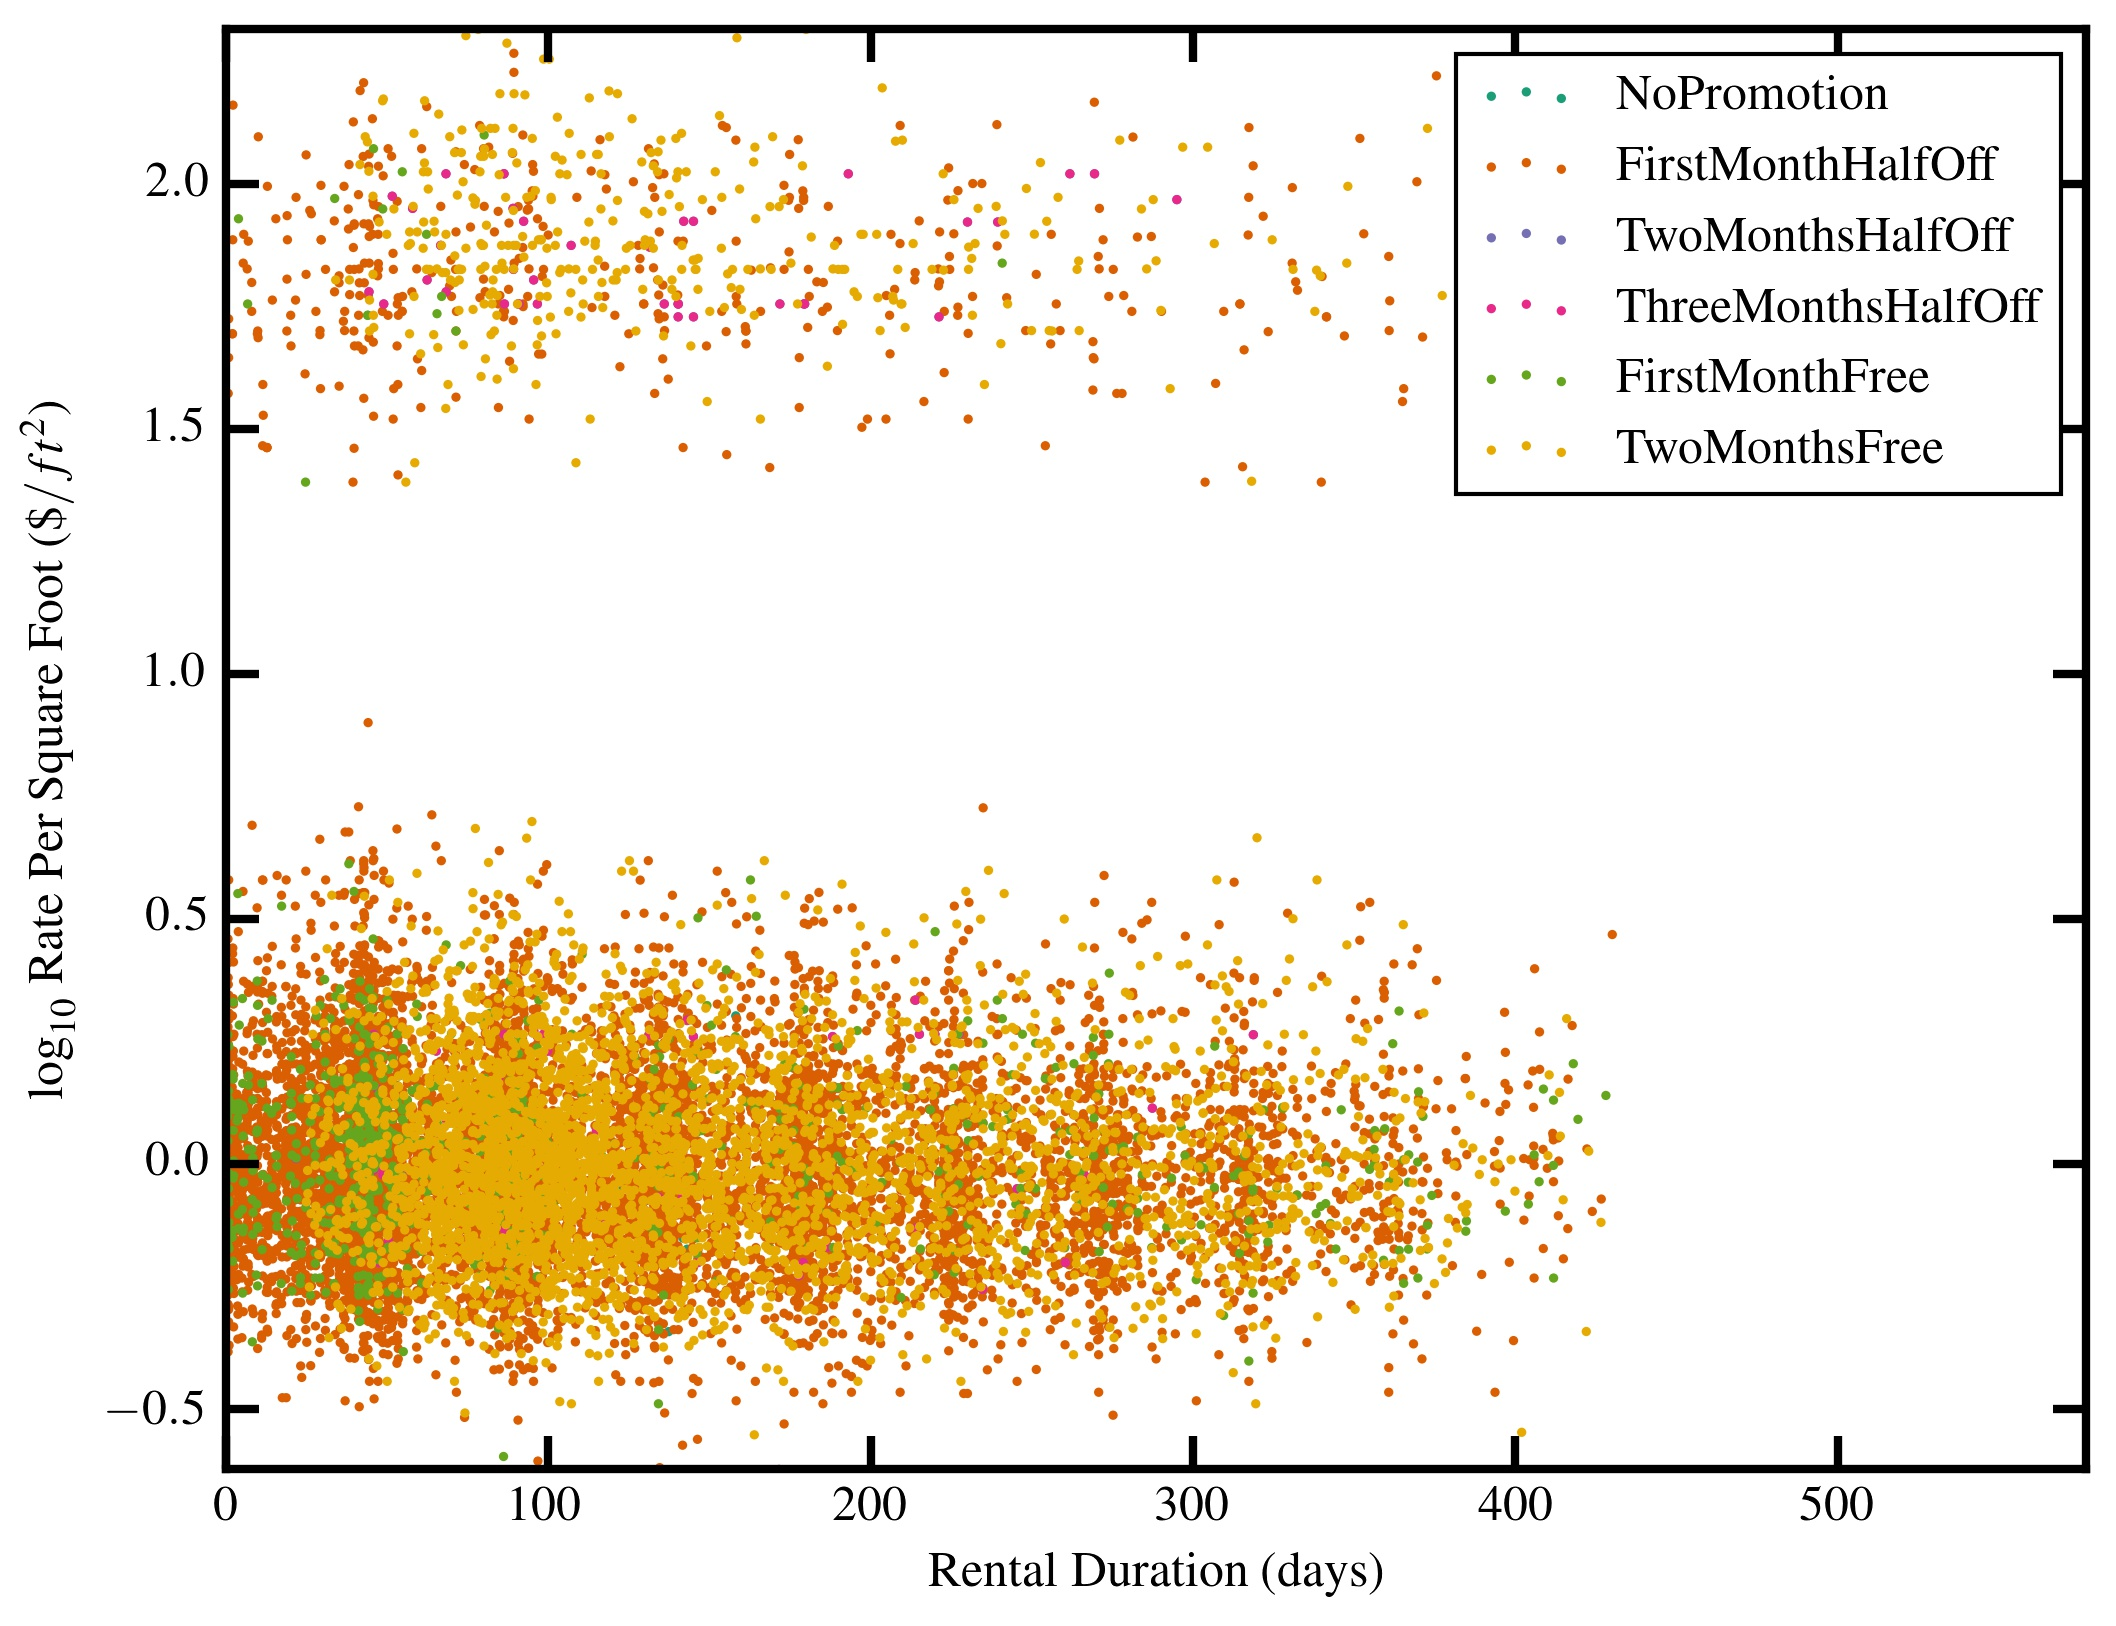
\includegraphics[width=0.9\columnwidth]{plots/FootRateVSDurations.jpg}
    \caption{Rental duration as a function of the rental rate per square foot. Each point is a single rental record and is colored by the type of promotion offered. Notice the weak trend in the rental duration as the rental rate per square foot varies. Also significant is the slight clustering in rental duration by promotion type suggesting that the rental duration may depend on the promotion type offered.}
    \label{fig:FootRateVSDuration}
\end{figure}

\begin{figure}
	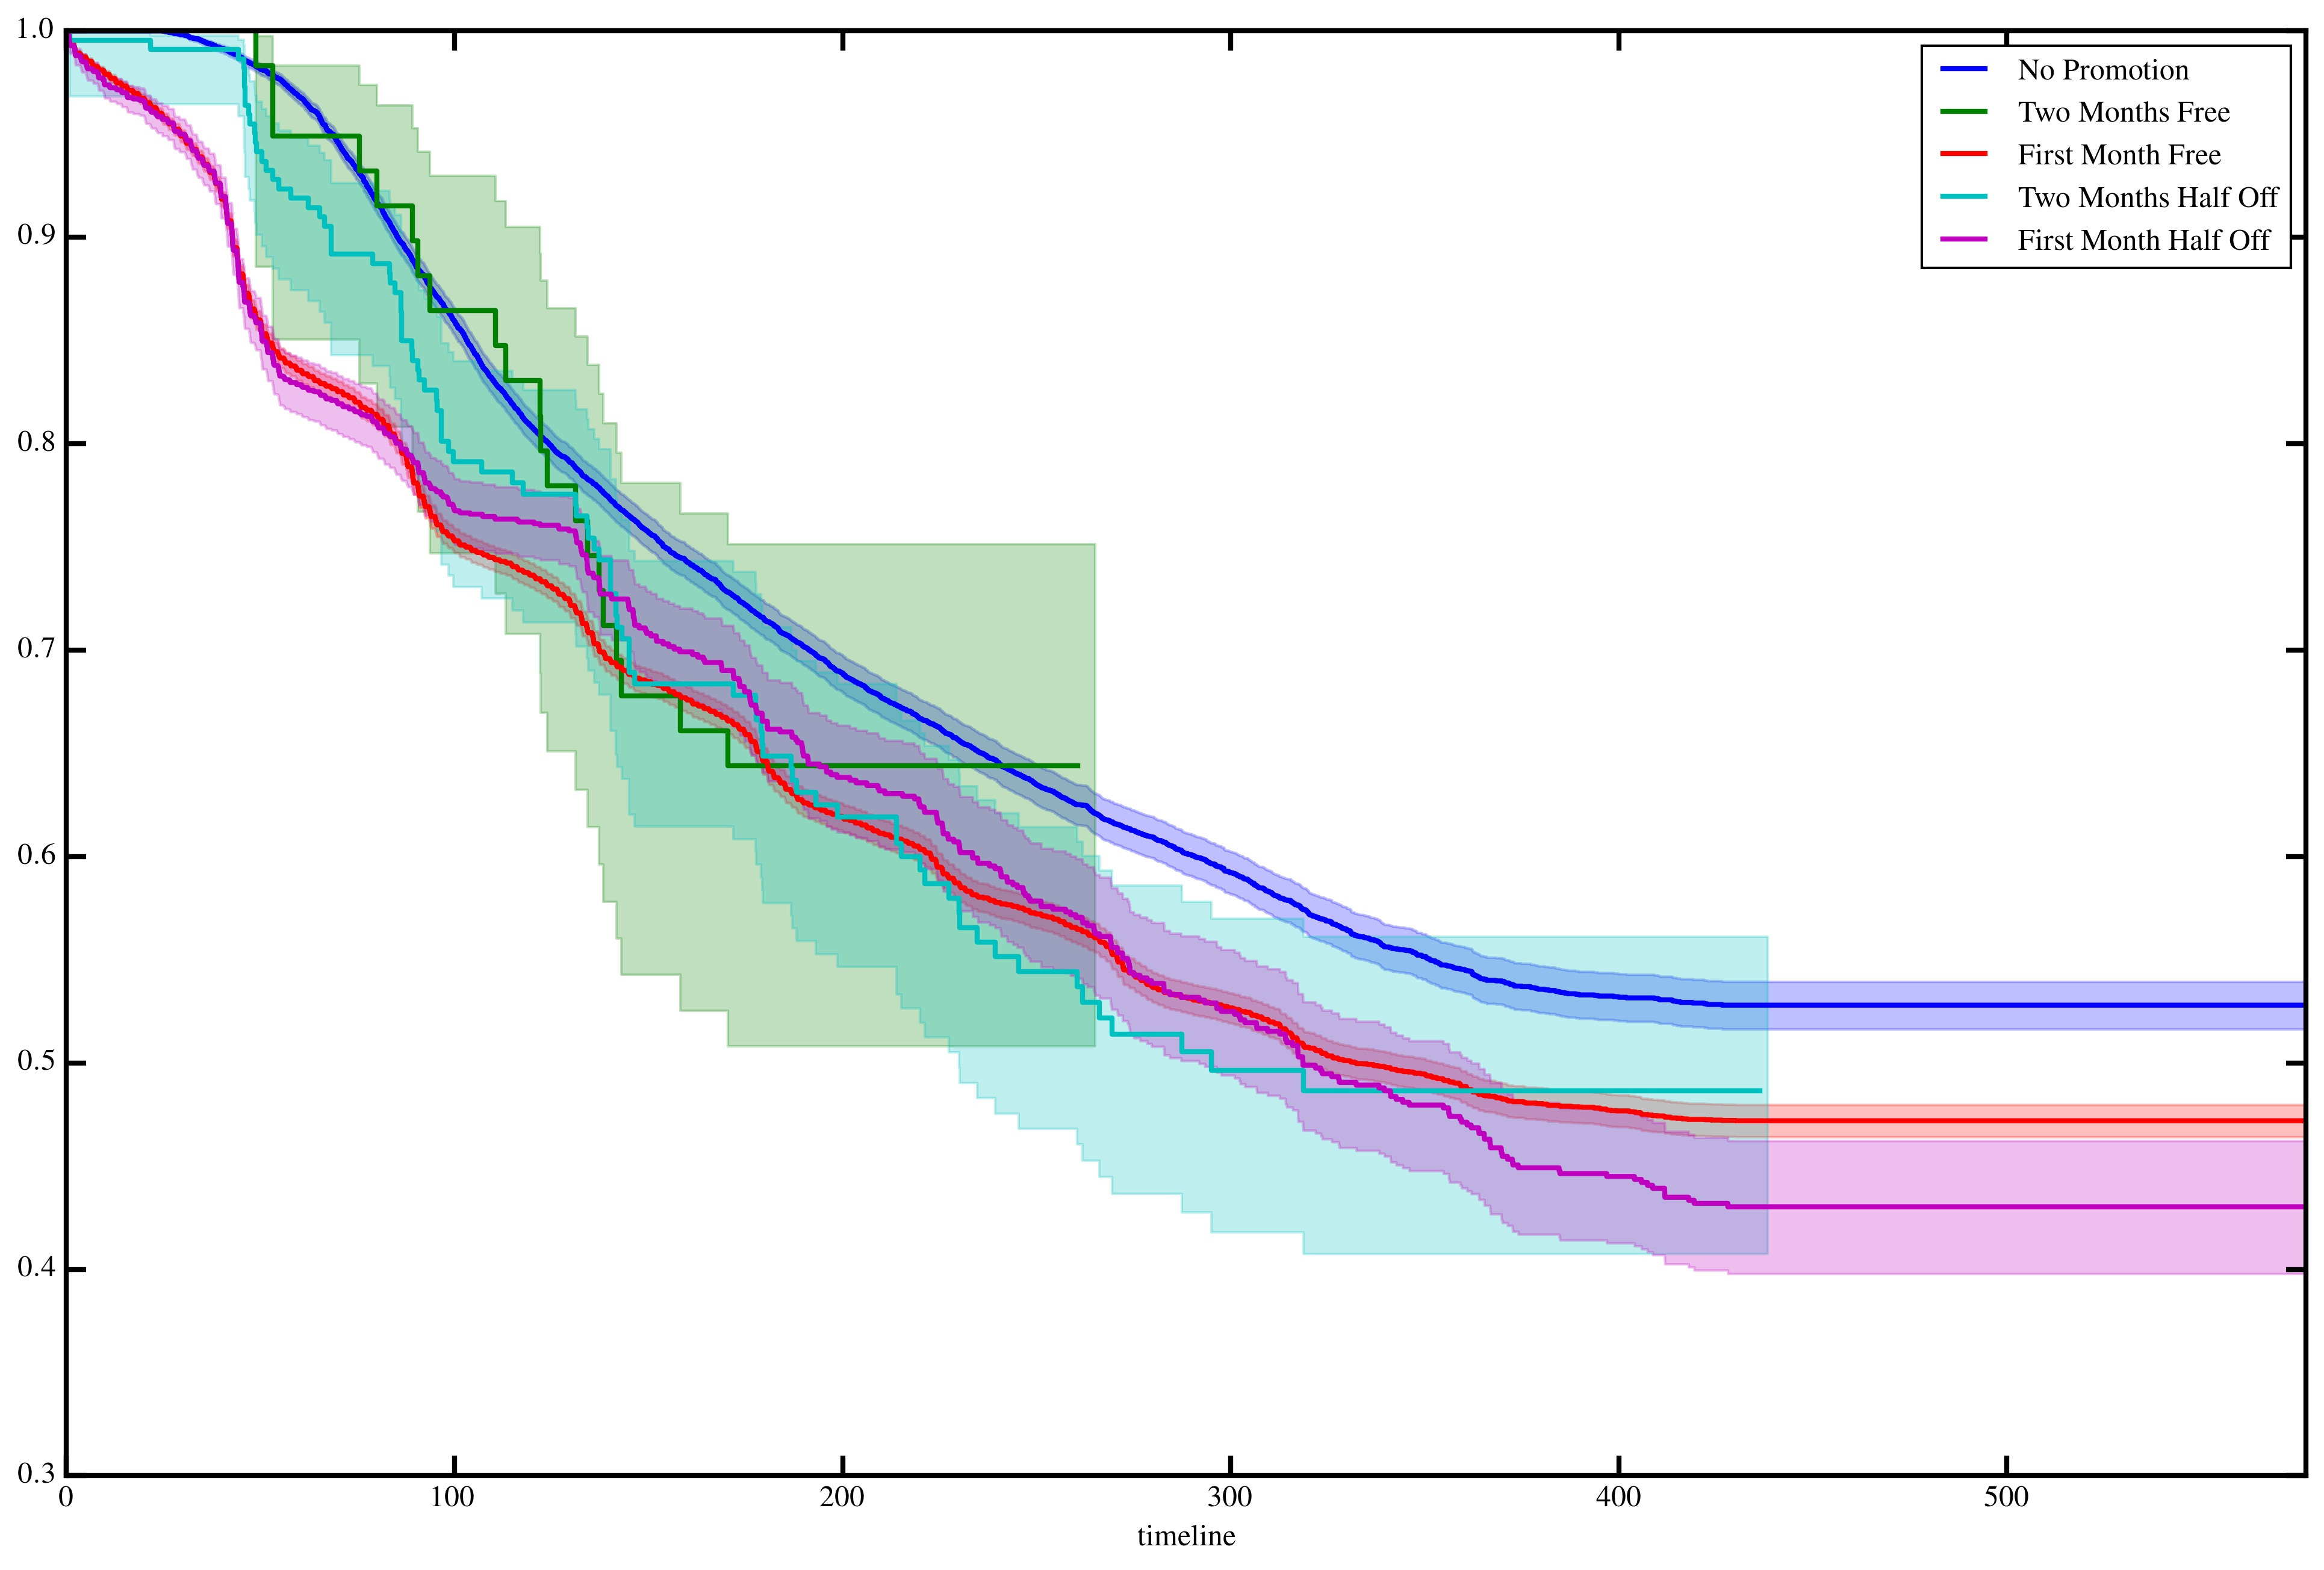
\includegraphics[width=0.9\columnwidth]{plots/DurationsSurvival_Breakdown_Overlaid.jpg}
    \caption{Survival functions for customers renting units with different kinds of promotions. The y-axis plots the likelihood that a customer will no longer be renting a storage unit after x-axis time $t$. In some cases, we have insufficient data to compute the survival functions down to the $50\%$ likelihood level. In such cases, we use a smoothing spline to estimate the rental duration at which there is a $50\%$ chance that the customer is still renting with CubeSmart.}
    \label{fig:SurvivalFunctions}
\end{figure}

\begin{figure}
	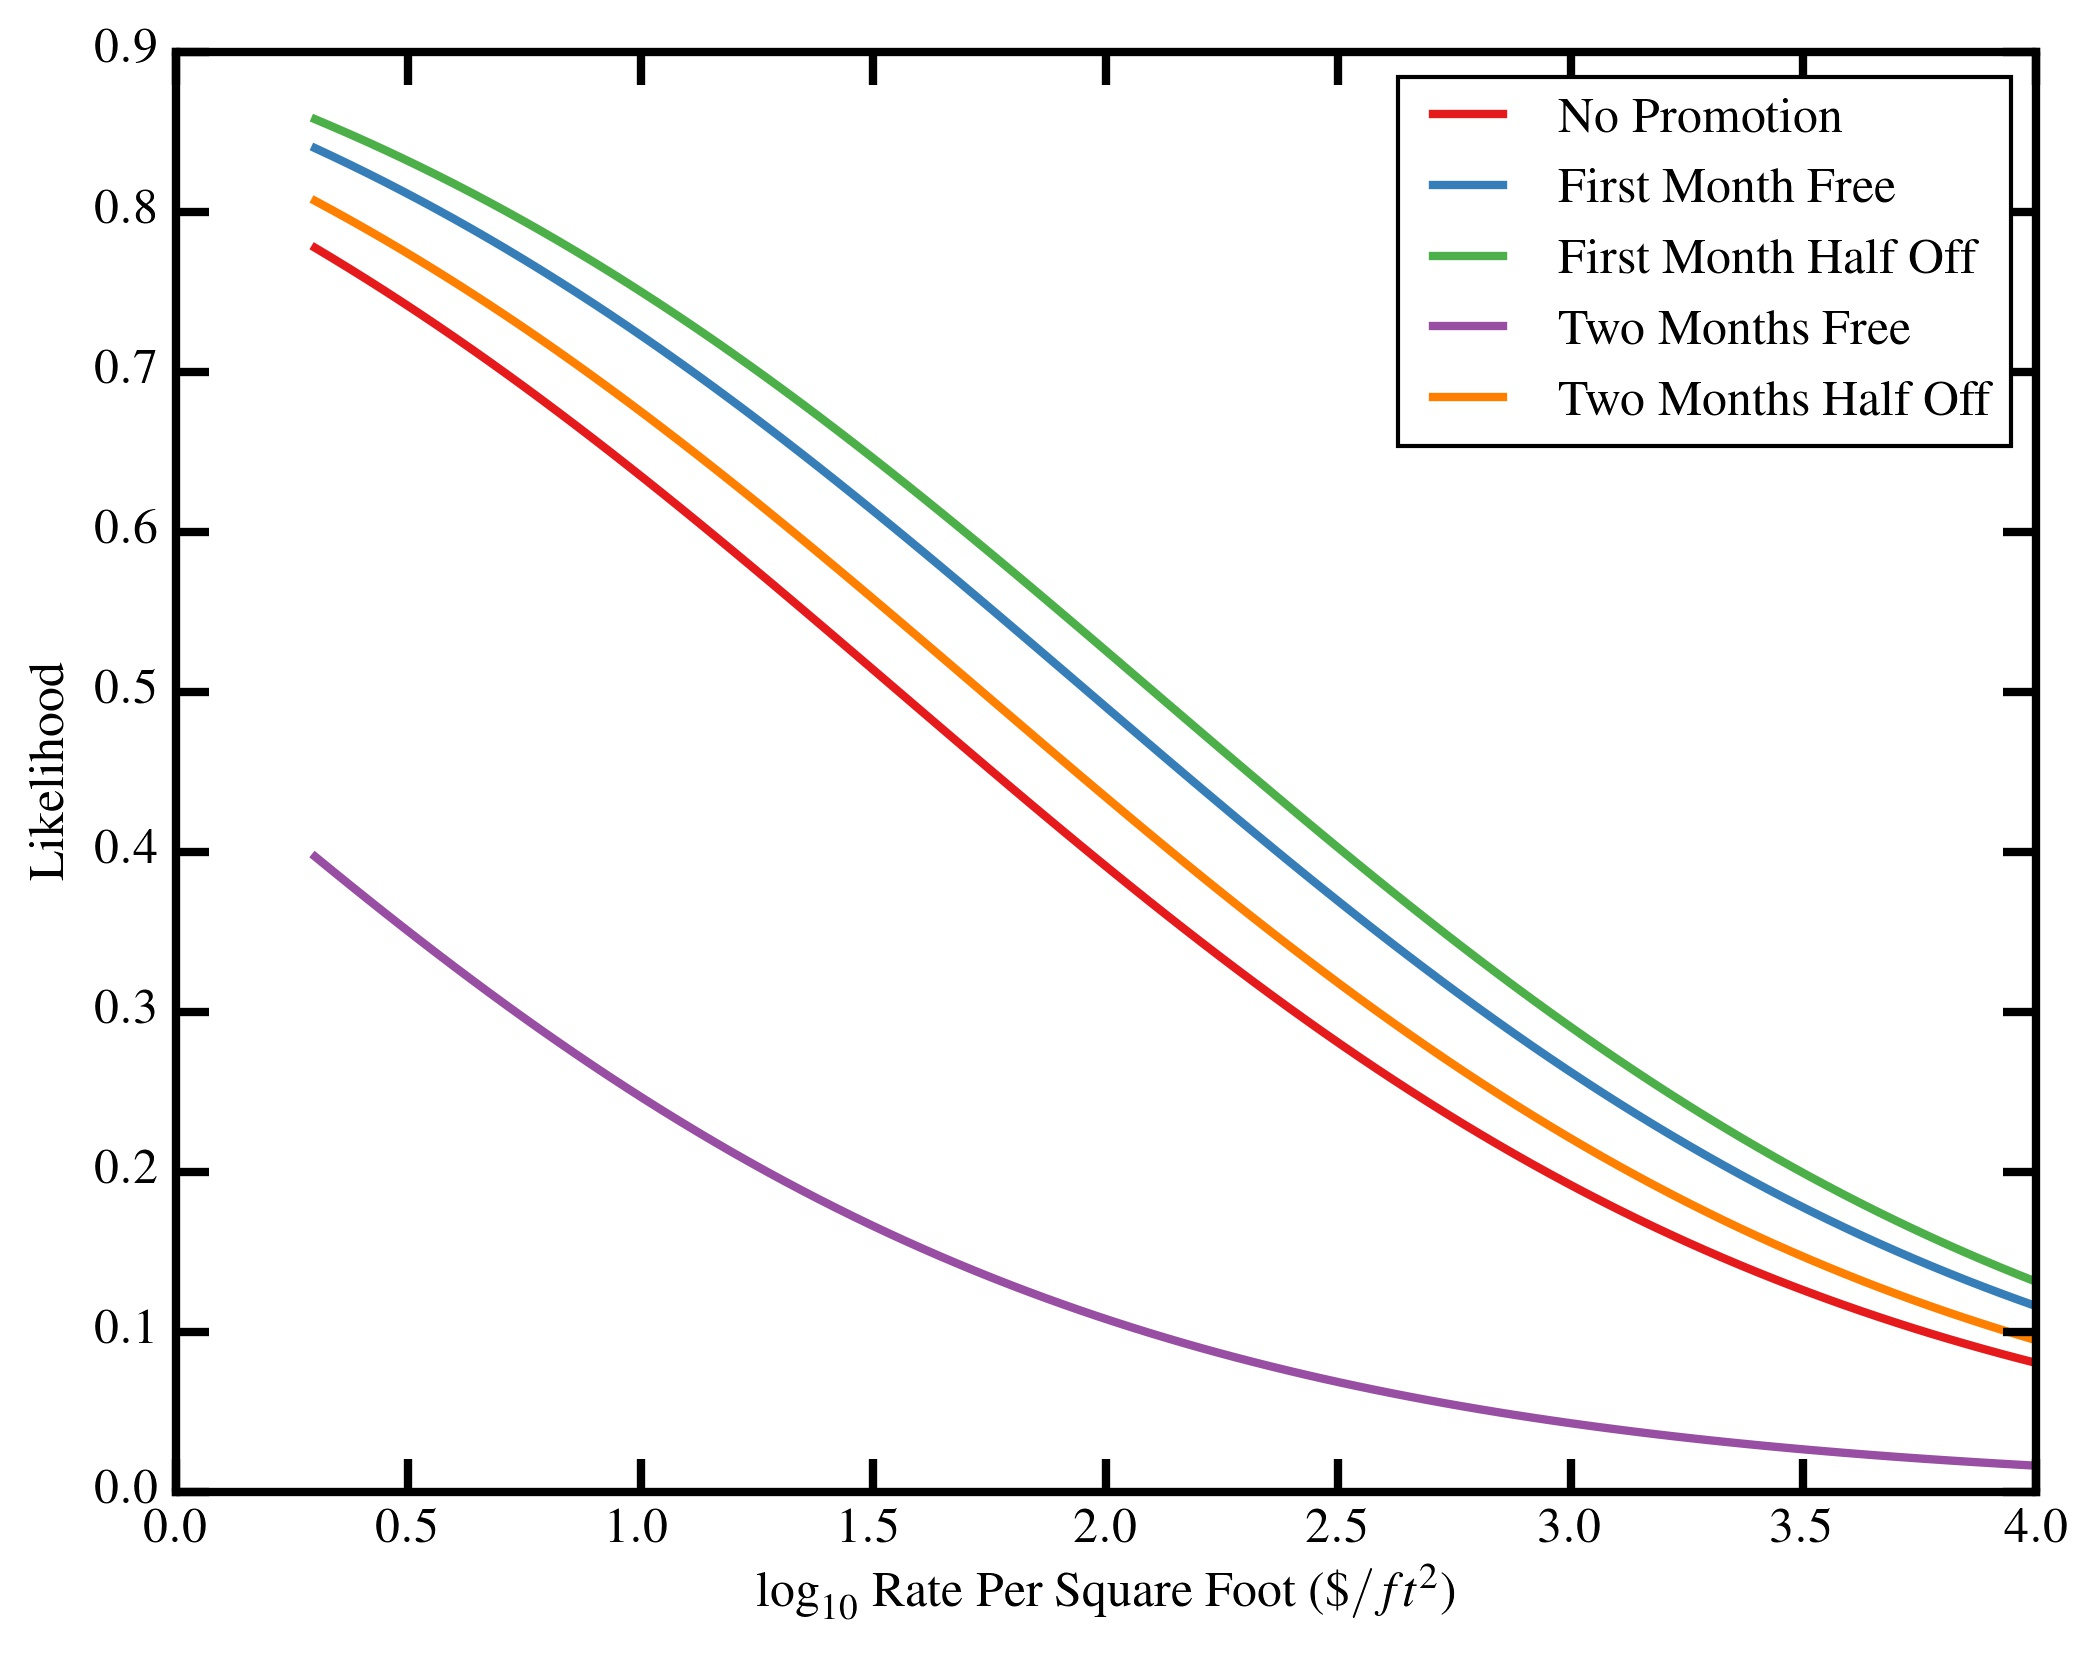
\includegraphics[width=0.9\columnwidth]{plots/ProbabilityCurve.jpg}
    \caption{Likelihoods of a customer renting a unit after making a reservation as a function of the cost per square foot.}
    \label{fig:ProbabilityCurve}
\end{figure}

\begin{figure}
	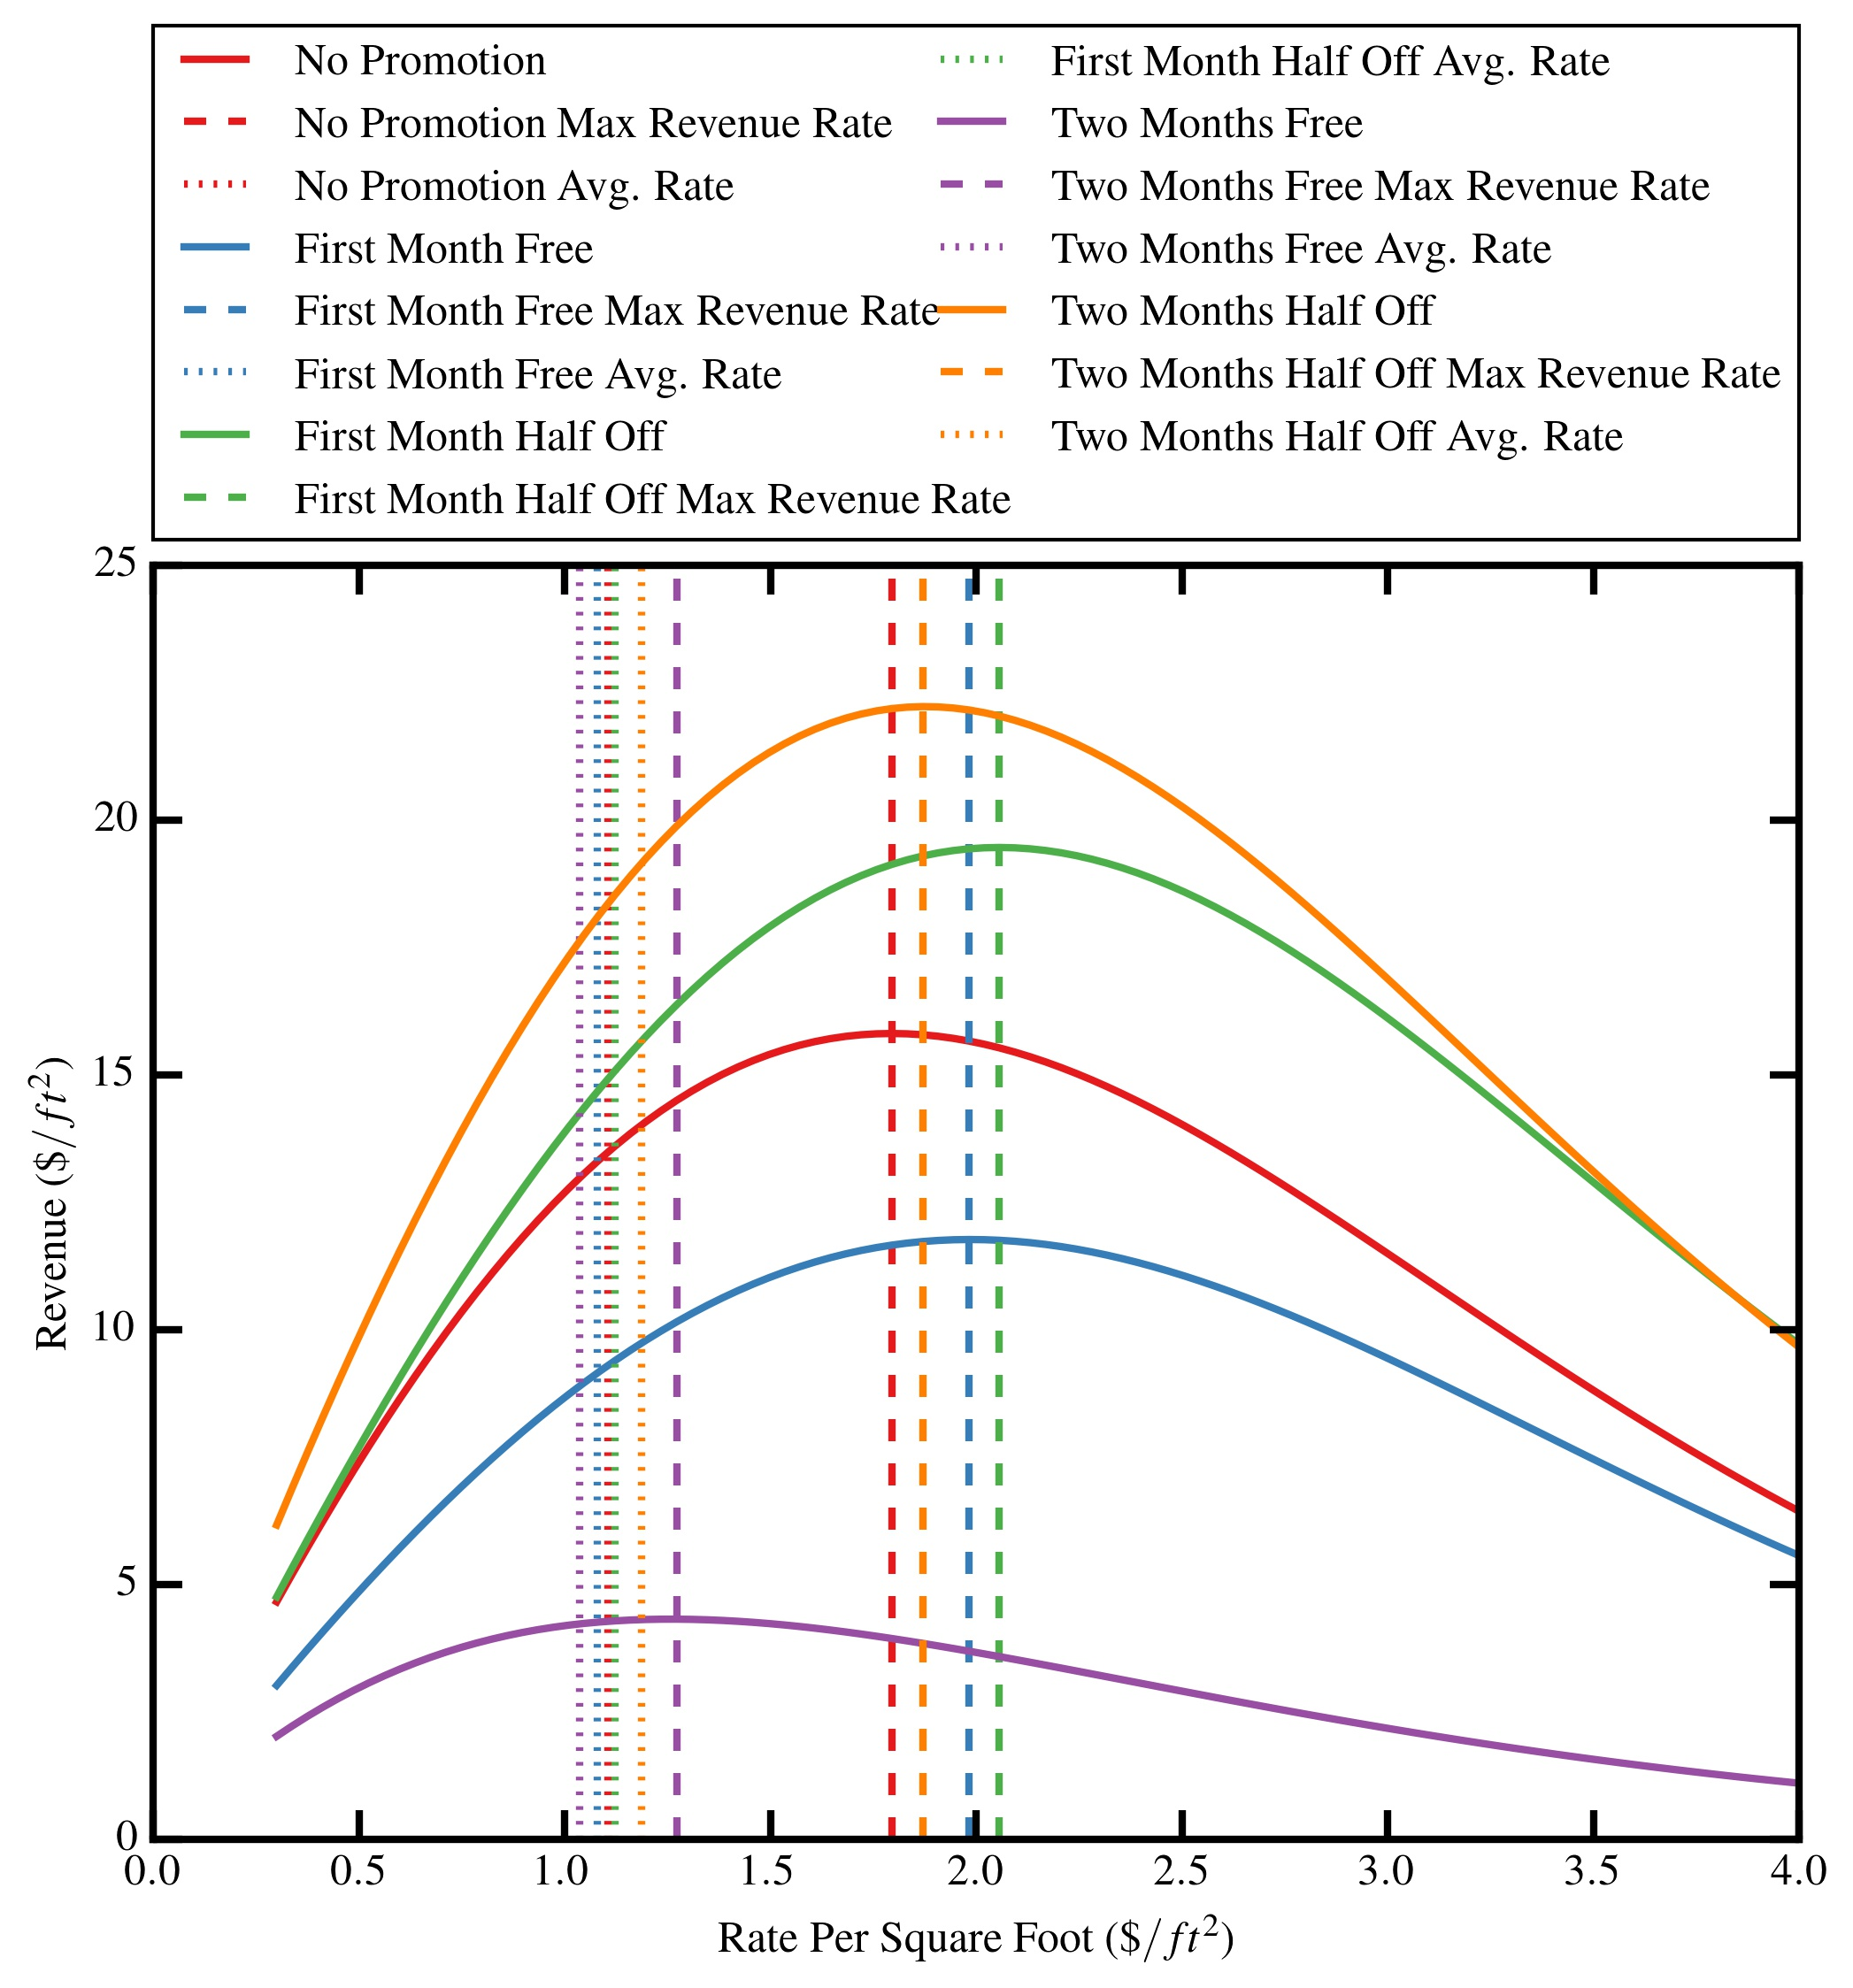
\includegraphics[width=0.9\columnwidth]{plots/RevenueCurve.jpg}
    \caption{Revenue $R$ generated by rentals as function of the rental rate per square foot $\rho$.}
    \label{fig:RevenueCurve}
\end{figure}

\end{document}

%% End of file `sample.tex'.
